\chapter{Definizioni}

\begin{definizione}[Multilayer network] 
    \label{def:muln}
    Una \muln\ è una coppia $(\mathcal{G}, \mathcal{E} )$ dove
    $\mathcal{G} = \{G_i \mid i \in \{1, 2, \dots L\}\}$ è un insieme di grafi
    detti \layer\ dove un nodo può appartenere ad uno o più layer ed 
    $\mathcal{E} = \{E_{ij} \subseteq V_i~\times~V_j \mid i,j \in \{1, 2, \dots, L\}, i \neq j\}$
    è l'insieme delle \interc\ tra nodi appartenenti a layer differenti.
\end{definizione}
% \begin{figure}
%     \centering
%     \def\svgwidth{\columnwidth}
%     \def\svgheight{\columnwidth}
%     \input{img/mlexample.pdf_tex}
% \end{figure}

% 

\begin{definizione}
    Data una multilayer network $\mathcal{M}=(\mathcal{G}, \mathcal{E})$ 
    indichiamo con $|V|$ il numero totale di nodi, ossia la cardinalità dell'insieme $V = \bigcup\limits_{i} V_i$,
    con $N$ la somma del numero di nodi di ogni layer, ossia $N = \sum_{i}{|V_i|}$
    e con $E$ il numero totale di archi, $E = \sum_{i} |E_i| + \sum_{i \neq j} |E_{ij}|$.    
\end{definizione}

\begin{definizione}[Multiplex network] 
    \label{def:mulx}
    Una \mulx\ è un tipo di multilayer network dove le uniche inter-connessioni ammesse sono tra un 
    nodo e le sue controparti negli altri layer, ossia 
    $E_{ij} \subseteq \{ (v,v) \mid v \in {V_i \cap V_j} \} $
\end{definizione}



\begin{definizione}[Grafo aggregato] 
    \label{def:gragg}
    Sia $\mathcal{M} = (\mathcal{G}, \mathcal{E} )$ una multilayer network. 
    Il \gragg\ derivato da $\mathcal{M}$ è il grafo 
    $G_{\mathit{agg}} = (V_{\mathit{agg}}, E_{\mathit{agg}})$  dove $V_{\mathit{agg}} = V$ ed 
    $E_{\mathit{agg}} = \biggl( \bigcup\limits_{i} E_{i} \biggr) \cup 
                    \biggl( \bigcup\limits_{i \neq j} E_{ij} \biggr)$
\end{definizione}

\begin{figure}[h]
    \centering
    \includegraphics[height=0.3\textheight]{img/definitions/mlexample.pdf}
    \caption{Rappresentazione di una multilayer network con tre layer: L1, L2 e L3.
    In rosso sono evidenziate le inter-connessioni, ossia gli archi che collegano nodi in 
    layer differenti.}
    \label{fig:mlexample}
\end{figure}

\begin{figure}
    \centering
    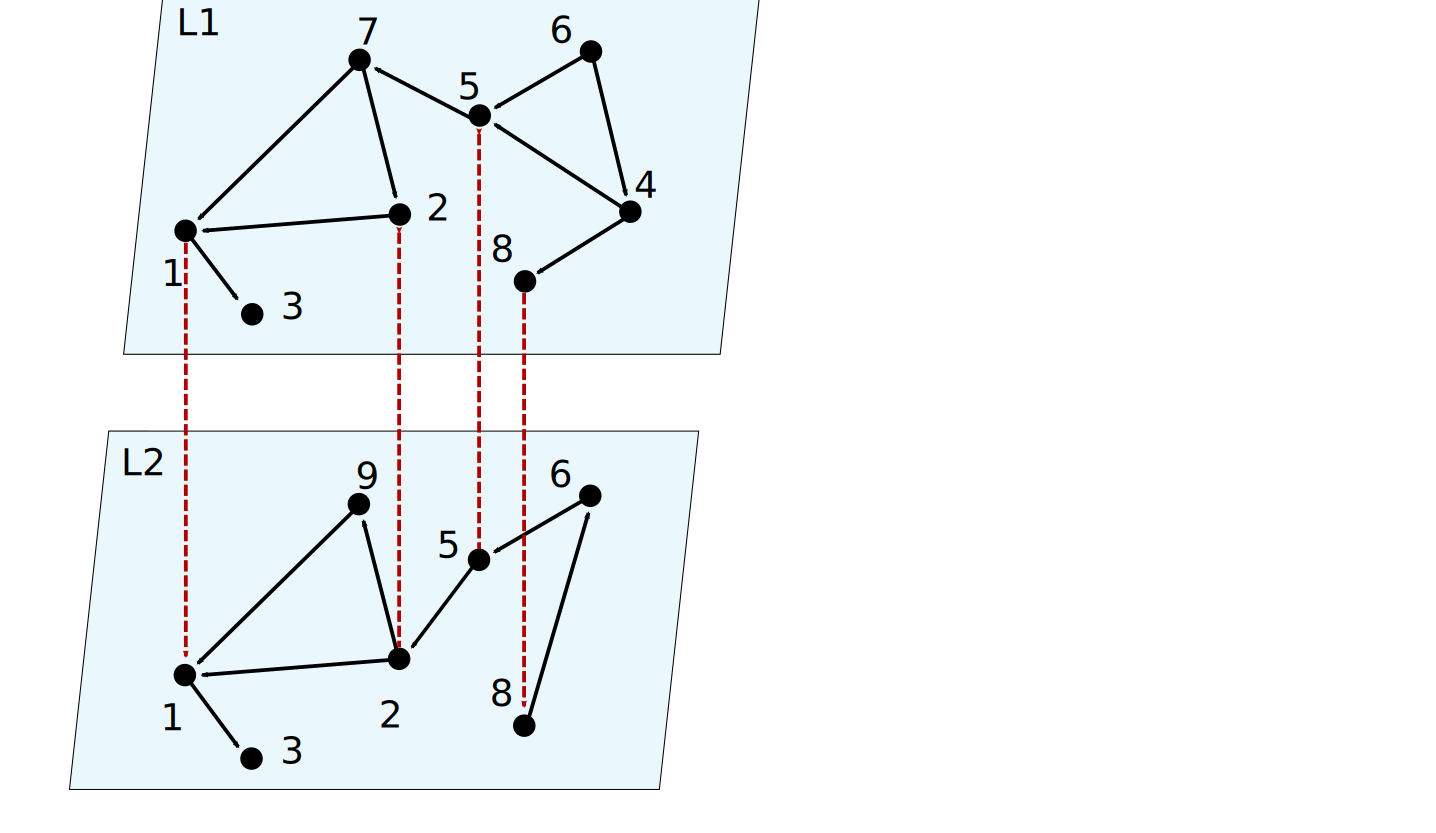
\includegraphics[height=0.3\textheight]{img/definitions/muxexample.pdf}
    \caption{Rappresentazione di una multiplex network con due layer: L1 e L2. In questo 
    tipo di rete le uniche inter-connessioni possibili sono tra un nodo e le sue controparti 
    negli altri layer.}
    \label{fig:muxexample}
\end{figure}

% 15865384615384615
\begin{figure}
    \centering
    \includegraphics[height=0.15865384615384615\textheight]{img/definitions/aggexample.pdf}
    \caption{Grafo aggregato derivato dalla multilayer network rappresentata in Figura \ref{fig:mlexample}.}
    \label{fig:graggexample}
\end{figure}
%[height=0.15865384615384615\textheight]
